% 2018 江苏卷第4题：算法伪代码框
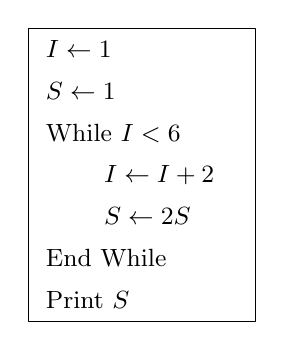
\begin{tikzpicture}[line cap=round,line join=round,font=\small,x=0.03515cm,y=0.03515cm]
\draw (0,0) rectangle (82,106);
\node[anchor=base west,inner sep=0] at (6.18,95.46) {\(I\leftarrow 1\)};
\node[anchor=base west,inner sep=0] at (6.18,80.34) {\(S\leftarrow 1\)};
\node[anchor=base west,inner sep=0] at (6.18,65.22) {While \(I<6\)};
\node[anchor=base west,inner sep=0] at (27.18,50.10) {\(I\leftarrow I+2\)};
\node[anchor=base west,inner sep=0] at (27.18,34.98) {\(S\leftarrow 2S\)};
\node[anchor=base west,inner sep=0] at (6.18,19.86) {End While};
\node[anchor=base west,inner sep=0] at (6.18,4.74) {Print \(S\)};
\end{tikzpicture}
